%%%%%%%%%%%%%%%%%%%%%%%%%%%%%%%%%%%%%%%%
\begin{figure}[thb]
\centering
% 
\begin{subfigure}[b]{0.45\linewidth}
\centering
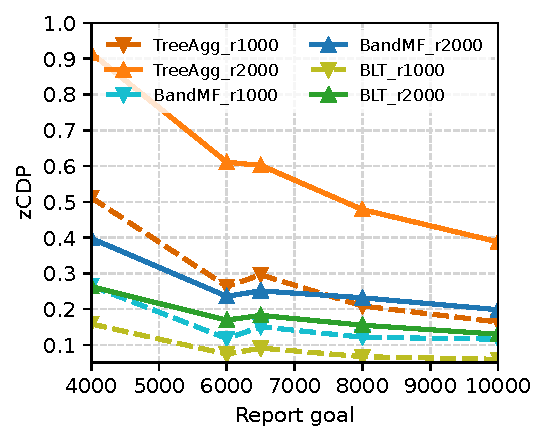
\includegraphics[width=\textwidth]{images/blt_pop3m.pdf}
\caption{\small Population 3M}
\label{fig:pop3m}
\end{subfigure}
%
\begin{subfigure}[b]{0.45\linewidth}
\centering
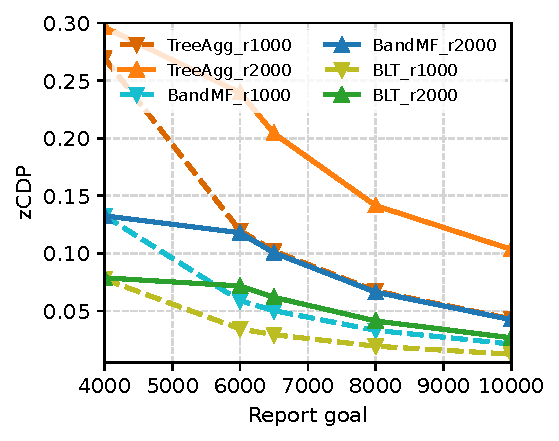
\includegraphics[width=\textwidth]{images/blt_pop10m.pdf}
\caption{\small Population 10M}
\label{fig:pop10m}
\end{subfigure}
%
\begin{subfigure}[b]{0.45\linewidth}
\centering
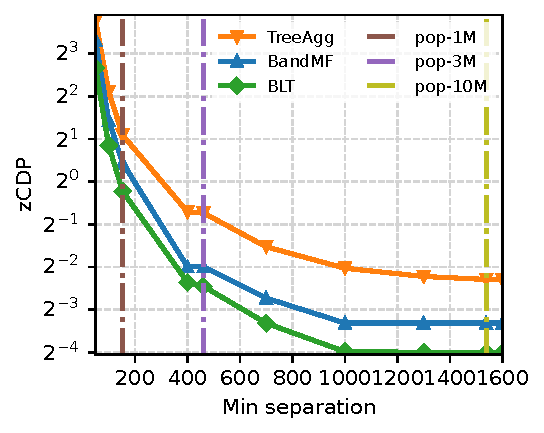
\includegraphics[width=\textwidth]{images/blt_min_sep.pdf}
\caption{\small Report goal 6500, worst-case max-par}
\label{fig:min_sep}
\end{subfigure}
%
\begin{subfigure}[b]{0.45\linewidth}
\centering
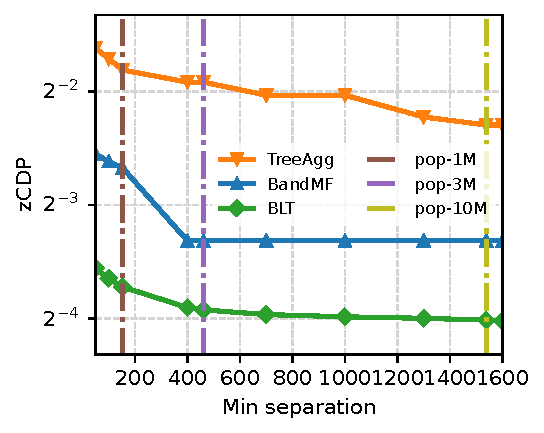
\includegraphics[width=\textwidth]{images/min_sep_max2.pdf}
\caption{\small Report goal 6500, optimistic max-par=2}
\label{fig:min_sep_max2}
\end{subfigure}
%
\caption{\small The effect of population size, number of rounds, report goals, and min-seps on DP-FTRL privacy guarantees. The results are extrapolate from the setting for es-ES and id-ID (\bandmf and \blt matrices are optimized for min-sep=400) based on the hypothesis that linearly scale noise multiplier and report goal, or only change min-sep will not affect the model utility. The For a fixed number of rounds to achieve utility target, increasing report goal and min-sep can achieve stronger guarantees measured by smaller zCDP. The optimal min-sep is capped by population size for a fixed report goal, and \blt provides better guarantees, and smoother transition across different min-seps. 
}\label{fig:extrapolate}
\end{figure}
%%%%%%%%%%%%%%%%%%%%%%%%%%%%%%%%%%%%%%%%

\paragraph{Extrapolation} We extrapolate the results for production setting by using a common hypothesis: linearly increase report goal and noise multiplier will not change the utility of the model as the signal-to-noise ratio is maintained. In addition, we assume only changing min-sep will not change the utility because of the signal-to-noise ratio. The hypothesis has been verified in previous work~\citep{kairouz21practical} and the large report goal experiments for pt-BR and pt-PT in \cref{tab:gboard} and \cref{fig:acc_curve}. Hence we can study the effect on DP without actually training the model, similar to \cref{sec:rmse_exp} for simulation.

We vary the report goal, and the min-sep is optimistically estimated by \emph{min-sep=$\lfloor$population-size/report-goal$\rfloor$}, and \emph{max-par=$\lceil$total-rounds/min-sep$\rceil$} is used unless otherwise specified. We discuss the extrapolation results in \cref{fig:extrapolate}, where utility is the same based on the hypothesis.
\begin{enumerate*}[label=\color{purple}(\arabic*)]
\item \blt achieves better DP guarantees because of its robustness to min-seps and total rounds. 
\item We observe that using larger report goal and optimizing for the largest possible min-sep achieves better results than using smaller report goals and larger corresponding min-sep, similar to observation for \treeagg in \citep{xu2023federated}.
\item \cref{fig:pop10m} shows training more rounds does not necessarily increasing DP guarantees when min-sep is large.
\item The gap of \blt and \bandmf is small when min-sep is accurately estimated. In the regime of relatively high signal-to-noise ratio (large noise multiplier for limited computation resources), \blt is competitive in a wide range of different configurations. Hence \blt is easier to use in production FL systems compared to \bandmf, and also saves memory during training.
\end{enumerate*}

Finally, in \cref{fig:varyn}, we extrapolate the DP guarantee results by varying the number of total rounds $n$ with the noise multiplier for the fixed report goal $6500$, fixed min separation $b=100,400,1000$, and corresponding max participation $k= n / b$. The \treeagg, \blt and \bandmf mechanisms used in production are compared. Instead of using \rmsloss or \maxloss to measure privacy-utility trade-offs in \cref{fig:rmse,fig:rmse_vary_n}, here we fix utility based on empirical utility of the production training and the signal-to-noise-ratio hypothesis, and compare the DP guarantees. As mentioned before, using \bandmf beyond the optimized matrices for $n=2000$ has not been studied before, and hence we only extrapolate \bandmf up to $n=2000$ rounds. \treeagg and \blt can run arbitrary number of rounds, and \blts achieve stronger DP guarantees than \treeagg. In practice, we can use one of the BLTs as a default mechanism across different settings, and perform on-the-fly optimization for given customized setting.  

\begin{figure}[thb]
\centering
\begin{subfigure}[b]{0.325\linewidth}
\centering
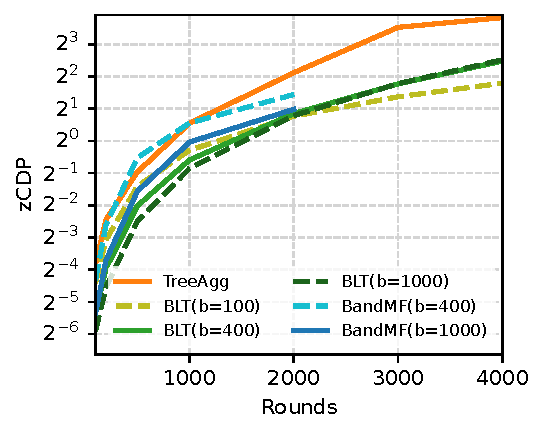
\includegraphics[width=\textwidth]{images/varyn_b100.pdf}
\caption{\small Min-sep b=100}
\label{fig:varyn_b100}
\end{subfigure}
%
\begin{subfigure}[b]{0.33\linewidth}
\centering
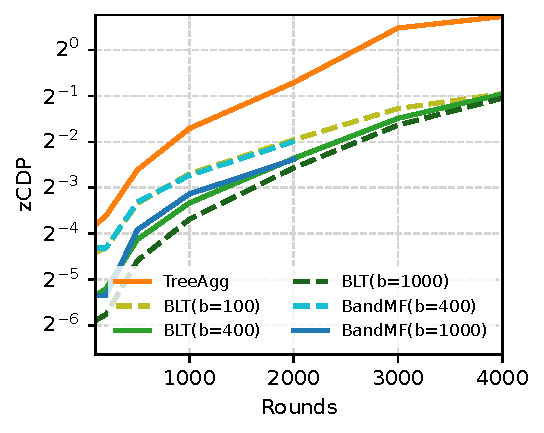
\includegraphics[width=\textwidth]{images/varyn_b400.pdf}
\caption{\small Min-sep b=400}
\label{fig:varyn_b400} 
\end{subfigure}
%
\begin{subfigure}[b]{0.33\linewidth}
\centering
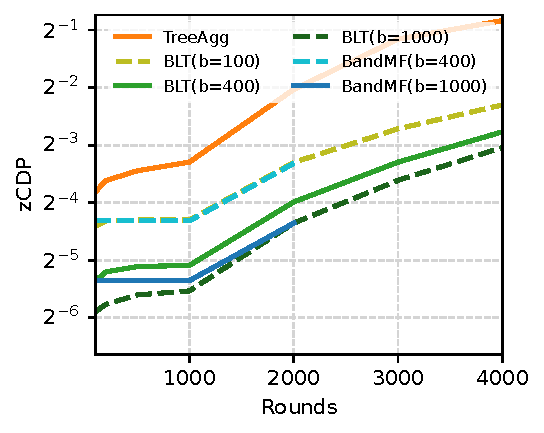
\includegraphics[width=\textwidth]{images/varyn_b1000.pdf}
\caption{\small Min-sep b=1000}
\label{fig:varyn_b1000} 
\end{subfigure}
%
\caption{\small Extrapolate by varying number of rounds $n$ for the \treeagg, \blt and \bandmf mechanisms used in production. Use the noise multiplier for the fixed report goal $6500$; fix min separation $b=100,400,1000$, respectively; worst-case max participation is varied assuming fixed population size, i.e., $k= n / b$. The utility of different mechanisms at a specific round (x-axis value) are assumed to be similar due to the signal-to-noise ratio hypothesis, and we can compare the corresponding zCDP guarantees (y-axis value).}\label{fig:varyn}
\end{figure}

\paragraph{Model launches} We have launched several language models for on-the-fly (OTF) rescoring words in Gboard smart completion and suggestion~\citep{gboard_dp_blogpost,xu2023federated}. The models trained with BLT-DP-FTRL algorithm in this paper achieved better privacy-utility trade-off than the \treeagg-DP-FTRL algorithm~\citep{kairouz21practical} widely used in FL practice~\citep{xu2023federated}, and comparable with MF-DP-FTRL~\citep{choquette2023amplified} that achieves state-of-the-art performance and some $\epsilon<1$ models reported in~\citep{gboard_dp_blogpost}. We report $\rho$-zCDP and $(\epsilon, \delta)$-DP of $\delta=10^{-10}$ following~\citet{xu2023federated,gboard_dp_blogpost}; the details of the DP configuration are provided in \cref{app:privacy-guarantees}. The Portuguese OTF LM in Brazil (pt-BR) is launched with DP $\epsilon=1.234$ (alternatively, zCDP $\rho=0.022$);
pt-PT OTF LM is launched with DP $\epsilon=8.19$ (alternatively, zCDP $\rho=0.749$) compared to DP $\epsilon=9.56$ (alternatively, zCDP $\rho=0.99$) in~\citep{xu2023federated}, and significant improvement in WMR of $-0.91\%$; 
es-ES OTF LM is launched with DP $\epsilon=4$ (alternatively, zCDP $\rho=0.202$) compared to DP $\epsilon=9.01$ (alternatively, zCDP $\rho=0.89$) in~\citep{xu2023federated}; the id-ID OTF LM using new vocabulary constructed from~\citep{gboard_fa_blogpost} is launched with DP $\epsilon=2.74$ (alternatively, zCDP $\rho=0.099$), achieving comparable utility and replacing the previous model without DP. In addition, the discussed default BLT mechanism optimized for $b=400$ and noise multiplier 7.379 is used to train and launch more models: the English LM is launched with DP $\epsilon=4.84$ (alternatively, zCDP $\rho=0.29$); the Spanish LM in Argentina is launched with DP $\epsilon=5.73$ (alternatively, zCDP $\rho=0.392$); the Spanish LM in Mexico is launched with DP $\epsilon=11.58$ (alternatively, zCDP $\rho=1.39$); the Spanish LM in other Latin America countries is launched with  DP $\epsilon=6.84$ (alternatively, zCDP $\rho=0.54$). The new Gboard OTF LMs are trained with FL and DP following the commitment in \citep{gboard_dp_blogpost,zhang2023private}. As of May 2025, all existing FL LMs have been replaced with DP FL models, fully realizing our plan in~\citep{zhang2023private}. 